\documentclass[11pt]{amsart}
\usepackage[a4paper,textwidth=158mm,textheight=237mm,centering]{geometry}
\usepackage[T1]{fontenc}
\usepackage{lmodern,microtype,mathtools,amssymb,graphicx,flafter,booktabs}
\usepackage[unicode,colorlinks=true,linkcolor=black,citecolor=black,urlcolor=blue]{hyperref}
\newtheorem{theorem}{Theorem}[section]
\newtheorem{lemma}[theorem]{Lemma}
\newtheorem{proposition}[theorem]{Proposition}
\newtheorem{corollary}[theorem]{Corollary}
\theoremstyle{remark}
\newtheorem{remark}[theorem]{Remark}
\title{Three phylogenetic trees on fourteen leaves always share a quartet}
\author{Harvey Yorke}
\address{Valyu AI}
\ifdefined\journalversion\else
\author{Valyu DeepResearch}
\address{Valyu AI}
\fi
\ifdefined\journalversion
  \hypersetup{pdftitle={Three phylogenetic trees on fourteen leaves always share a quartet},pdfauthor={Harvey Yorke}}
\else
  \hypersetup{pdftitle={Three phylogenetic trees on fourteen leaves always share a quartet},pdfauthor={Harvey Yorke and Valyu DeepResearch}}
\fi
\date{25 October 2026}
\keywords{Phylogenetic trees, quartets, agreement subtrees, separators, caterpillars, SAT certificates}
\newcommand{\paperAuthorBlock}[1]{%
  \begin{minipage}[t]{.44\textwidth}
    \centering\normalfont\normalsize #1\par\small Valyu AI\par
  \end{minipage}%
}
\makeatletter
\renewcommand{\@setauthors}{%
  \begingroup\trivlist\centering\normalfont\normalsize
  \@topsep30\p@\relax\advance\@topsep by -\baselineskip\item\relax
  \ifdefined\journalversion
    \paperAuthorBlock{Harvey Yorke}%
  \else
    \paperAuthorBlock{Harvey Yorke}\hspace{.06\textwidth}\paperAuthorBlock{Valyu DeepResearch}%
  \fi
  \endtrivlist\endgroup
}
\renewcommand{\@setaddresses}{}
\makeatother
\begin{document}
\raggedbottom
\begin{abstract}
Snir and Yuster asked for $h(k)$, the least $n$ such that any $k$ unrooted binary phylogenetic trees on the same $n$ leaves resolve some four leaves identically. It was known that $h(2)=6$ and $11\le h(3)\le14$; for general $k$ the upper bound was a four-fold iterated exponential. We prove $h(3)=14$. The lower bound is a tree $T$ on thirteen leaves and a leaf permutation $\sigma$ of order three such that $T$, $\sigma T$ and $\sigma^2T$ have no common quartet. For the upper bound we give an exact finite version of the Snir--Yuster argument: an exhaustive check over the $135$ tree shapes on fourteen leaves shows that a balanced edge of the first tree and a suitable edge of the second always leave separated leaf sets of sizes three and four, and a SAT computation with DRAT-checked certificates confirms the two-tree statement independently. Iterating the underlying balanced-cut step, balanced on the larger set and with the potential $\min\{|X||Y|,2|X|^2,2|Y|^2\}$, gives the elementary bound $h(k)\le\lfloor 3\beta^{k-1}\rfloor+1$ for all $k$, where $\beta=(1+\sqrt{13})/2$; done exactly by dynamic programming, the same bookkeeping gives $h(4)\le28$, $h(5)\le61$ and $h(6)\le125$. Together with the caterpillar families of Snir and Yuster, for which we give an explicit construction, this gives $2^k+2\le h(k)\le\lfloor 3\beta^{k-1}\rfloor+1$. A symmetric SAT construction gives $h(4)\ge23$, so $23\le h(4)\le28$.
\end{abstract}
\maketitle

\section{Introduction}

A \emph{phylogenetic tree} on $[n]=\{1,\dots,n\}$ is an unrooted tree whose internal vertices have degree three and whose leaves are labelled bijectively by $[n]$. Restricting a tree to a $4$-set $Q$ and suppressing degree-two vertices leaves one internal edge, which splits $Q$ into two pairs: the \emph{quartet split} $ab|cd$, $ac|bd$ or $ad|bc$. A family of trees on $[n]$ has a \emph{common quartet} if some $4$-set has the same split in every member. Let $h(k)$ be the least $n$ such that every $k$ trees on $[n]$ have a common quartet, and put $N(k)=h(k)-1$. Restricting all trees to a subset of the leaves preserves the absence of a common quartet, so $k$ trees without one exist on $n$ leaves exactly when $n\le N(k)$. Clearly $h(1)=4$ and $N(k)$ is nondecreasing in $k$.

Bandelt and Dress~\cite{BD1986} noted that two trees on at least six leaves share a quartet, so $h(2)=6$. Snir and Yuster~\cite[Sec.~5]{SY2026} introduced $h(k)$ and its caterpillar analogue $h^*(k)$, for which they state $h^*(k)=2^k+2$, remarked that determining $h(k)$ ``seems considerably more involved'', and showed $h(3)>10$ with three trees on ten leaves. Since caterpillars are phylogenetic trees, $h(k)\ge h^*(k)$; Snir and Yuster omit the construction behind $h^*(k)\ge2^k+2$, and we give one in Section~\ref{sec:lowerbounds}. Their theorem that any three trees on $n$ leaves have separated leaf sets of size at least $2n/27$~\cite[Thm.~1.3]{SY2026} gives $h(3)\le14$, as Currie, Czabarka, Fischer, Simmons, Sz\'ekely and Wicke observed~\cite{CCFSSW2026}, who also proved
\[
8^{1/4}3^{k/4}\le h(k)\le \operatorname{tw}_3\bigl(6(k-1)2^k+O(\log k)\bigr)
\]
through hypergraph Ramsey numbers~\cite[Thm.~5]{CCFSSW2026}.

\begin{theorem}\label{thm:h3}
$h(3)=14$.
\end{theorem}

\begin{theorem}\label{thm:general}
Put $\beta=(1+\sqrt{13})/2$. Then $2^k+2\le h(k)\le\lfloor 3\beta^{k-1}\rfloor+1$ for every $k\ge1$.
\end{theorem}

Theorem~\ref{thm:general} replaces the iterated exponential by a single exponential and pins the growth rate between $2$ and $\beta\approx2.3028$: $\log2\le\liminf_k\tfrac1k\log h(k)\le\limsup_k\tfrac1k\log h(k)\le\log\beta$. The lower bound is the caterpillar bound of Snir and Yuster; Currie et al.\ state the weaker $h(k)\ge8^{1/4}3^{k/4}$. The upper bound iterates the balanced-cut and pigeonhole steps that Snir and Yuster use for two and three trees (their Proposition~2.4 and the proof of Theorem~2.5) and for paths (their Proposition~5.2). The plain iteration gives $h(k)\le2\cdot3^{k-1}+1$ (Proposition~\ref{prop:plain}); what is new is the iteration for trees with exact bookkeeping, and the reduction of the base from $3$ to $\beta$ by balancing the cut on the larger set and tracking a potential instead of the smaller set (Lemma~\ref{lem:potential}). Done exactly, by dynamic programming over coloured trees, the same bookkeeping gives $h(4)\le28$, $h(5)\le61$ and $h(6)\le125$ (Theorem~\ref{thm:smallk}). Table~\ref{tab:small} collects small values.

\begin{table}[ht]
\centering
\begin{tabular}{rllll}
\toprule
$k$ & lower bound & source & upper bound & source \\
\midrule
1 & 4 & trivial & 4 & trivial \\
2 & 6 & \cite{BD1986} & 6 & \cite{BD1986} \\
3 & 14 & Proposition~\ref{prop:lower} & 14 & Theorem~\ref{thm:h3} \\
4 & 23 & SAT, $\sigma$ of type $4^52$ & 28 & Theorem~\ref{thm:smallk} \\
5 & 34 & caterpillars, Proposition~\ref{prop:cat} & 61 & Theorem~\ref{thm:smallk} \\
6 & 66 & caterpillars, Proposition~\ref{prop:cat} & 125 & Theorem~\ref{thm:smallk} \\
$k$ & $2^k+2$ & caterpillars, Proposition~\ref{prop:cat} & $\lfloor3\beta^{k-1}\rfloor+1$ & Theorem~\ref{thm:weighted} \\
\bottomrule
\end{tabular}
\caption{Bounds on $h(k)$ for small $k$. Before this note the bounds for $k=3$ were $11$ and $14$, and for $k\ge4$ the upper bounds were iterated exponentials. For $k=4$ the caterpillar bound is $18$.}
\label{tab:small}
\end{table}

\section{Separated sets}\label{sec:sep}

Disjoint leaf sets $X$ and $Y$ are \emph{separated} in a tree if some edge has all of $X$ on one side and all of $Y$ on the other. If $X$ and $Y$ are separated in every tree of a family and $x,x'\in X$, $y,y'\in Y$ are distinct, every tree resolves $\{x,x',y,y'\}$ as $xx'|yy'$, a common quartet.

\begin{lemma}[balanced edge]\label{lem:centroid}
Every phylogenetic tree with $m\ge2$ leaves has an edge with at least $m/3$ leaves on each side.
\end{lemma}

\begin{proof}
This is classical; we include the short argument. Choose an edge $uv$ minimising the larger number $M$ of leaves on one side, and let that side contain $v$. If $M>2m/3$ then $M\ge2$, so $v$ is internal and its two other edges cut the $M$ leaves into parts $a+b=M$ with $a,b\ge1$. The edge leading to the $a$ leaves has sides $a<M$ and $m-a$, so minimality gives $m-a\ge M$; likewise $m-b\ge M$. Adding, $2m-M\ge2M$, a contradiction.
\end{proof}

For a set $S$ of at least two leaves of $T$, the restriction $T|S$ is the tree spanned by $S$ with degree-two vertices suppressed. Each edge of $T|S$ comes from a path of $T$, and removing any edge of that path splits $S$ as the edge of $T|S$ does. So Lemma~\ref{lem:centroid} gives an edge of $T$ splitting $S$ into two parts with at least $|S|/3$ elements each.

\begin{lemma}[step]\label{lem:step}
Let $X,Y$ be separated in trees $T_1,\dots,T_j$, and let an edge of a further tree $T'$ split $X\cup Y$ into $W$ and $Z$. If $|X|,|Y|,|W|,|Z|\ge 2t-1$, then one of the pairs $(X\cap Z,\,Y\cap W)$ and $(X\cap W,\,Y\cap Z)$ consists of two sets with at least $t$ elements each. Both pairs are separated in $T_1,\dots,T_j,T'$.
\end{lemma}

\begin{proof}
Put $A=X\cap Z$, $B=X\cap W$, $C=Y\cap Z$ and $D=Y\cap W$. Subsets of $X$ and $Y$ remain separated in each $T_i$, and $A,C\subseteq Z$, $B,D\subseteq W$ are separated in $T'$. If $\min\{|A|,|D|\}\le t-1$ and $\min\{|B|,|C|\}\le t-1$, then one of $|A|+|B|=|X|$, $|A|+|C|=|Z|$, $|D|+|B|=|W|$, $|D|+|C|=|Y|$ is at most $2t-2$.
\end{proof}

\begin{proposition}\label{prop:plain}
$h(k)\le 2\cdot3^{k-1}+1$ for every $k\ge2$.
\end{proposition}

\begin{proof}
Let $\phi(s)=\lfloor(\lceil 2s/3\rceil+1)/2\rfloor$. If $X,Y$ are separated in some trees and $|X|,|Y|\ge s$, Lemma~\ref{lem:centroid} applied to $T'|(X\cup Y)$ gives $|W|,|Z|\ge\lceil 2s/3\rceil$, and $\lceil 2s/3\rceil\le s$, so Lemma~\ref{lem:step} with $t=\phi(s)$ produces a pair of size at least $\phi(s)$ separated in one more tree. Moreover $\phi(s)\ge a$ if and only if $\lceil 2s/3\rceil\ge 2a-1$, that is $s\ge 3a-2$. Define $b_1=2$ and $b_{i+1}=3b_i-2$, so $b_i=3^{i-1}+1$: a pair of size $b_i$ separated in some trees can be pushed through $i-1$ further trees and still have size at least $2$.

Let $T_1,\dots,T_k$ be trees on $n\ge 2\cdot 3^{k-1}+1$ leaves, $k\ge2$. Balanced edges of $T_1$ and of $T_2$ split $[n]$ into $X\cup Y$ and $W\cup Z$ with all four parts of size at least $\lceil n/3\rceil\ge 2\cdot3^{k-2}+1$. Lemma~\ref{lem:step} with $t=3^{k-2}+1=b_{k-1}$ gives a pair of size $b_{k-1}$ separated in $T_1,T_2$. Pushing it through $T_3,\dots,T_k$ yields two sets of size at least $2$ separated in all $k$ trees, hence a common quartet.
\end{proof}

\begin{remark}
For $k=2$ the bound is $7$ (the truth is $6$), and for $k=3$ it is $19$. The executable file \texttt{iterate\_check.py} runs this proof on random families at the threshold $n=2\cdot3^{k-1}+1$ for $k\le5$ and checks every intermediate size bound; it also runs the proof of Theorem~\ref{thm:weighted} below for $k\le6$, checking the potential with exact rationals.
\end{remark}

\subsection*{A smaller base}
Proposition~\ref{prop:plain} loses a factor $3$ per tree because it only tracks the smaller of the two sets. Balancing the cut on the larger set and tracking a potential does better.

\begin{lemma}[weighted balanced edge]\label{lem:weighted}
Let $T$ be a phylogenetic tree with at least two leaves, and give the leaves nonnegative weights with total $1$, each at most $1/2$. Then some edge of $T$ has weight at least $1/3$ on each side.
\end{lemma}

\begin{proof}
If some edge has weight at most $1/2$ on each side, both sides weigh $1/2$. Otherwise direct every edge towards its side of weight more than $1/2$. Two components of $T-v$ cannot both weigh more than $1/2$, so every vertex has at most one outgoing edge; as a tree has more vertices than edges, some vertex $v$ has none, so every component of $T-v$ weighs at most $1/2$. A leaf $v$ would then be a side of weight more than $1/2$ by itself, so $v$ is internal and its three components have total weight $1$. The heaviest weighs between $1/3$ and $1/2$, and the edge joining it to $v$ has weight at least $1/3$ on each side.
\end{proof}

For real $a,d\ge0$ put $\Psi(a,d)=\min\{ad,\,2a^2,\,2d^2\}$. It is symmetric, nondecreasing in each argument and homogeneous of degree two, and $\Psi(a,d)\le2\min\{a,d\}^2$.

\begin{lemma}[potential step]\label{lem:potential}
Put $t=(\sqrt{13}-1)/6$ and $c=t^2=(7-\sqrt{13})/18$. Let $0<a\le d$, $x\in[0,1]$ and $y\in[1/3,2/3]$. Then
\[
\max\bigl\{\Psi\bigl(xa,(1-y)d\bigr),\ \Psi\bigl((1-x)a,yd\bigr)\bigr\}\ \ge\ c\,\Psi(a,d).
\]
The constant $c$ is best possible for this real-variable inequality.
\end{lemma}

\begin{proof}
The constants satisfy $3t^2+t=1$, $0<t<1/2$ and $c<2/9$. Call the two terms $O_1$ and $O_2$. Replacing $(x,y)$ by $(1-x,1-y)$ exchanges them and preserves the hypothesis, so we may assume $x+y\le1$; by homogeneity $a=1$ and $d=r\ge1$. If $r>2$ then $\Psi(1,r)=\Psi(1,2)=2$ while $O_1,O_2$ only decrease when $r$ is lowered to $2$, so we may assume $1\le r\le2$, and the target is $c\Psi(1,r)=cr$.

\emph{Case $x\ge t$.} Since $1-y\ge x$, the three entries of $O_1$ satisfy
\[
x(1-y)r\ge x^2r\ge cr,\qquad 2x^2\ge2c\ge cr,\qquad
2(1-y)^2r^2\ge2cr^2\ge cr.
\]

\emph{Case $x<t$.} The three entries of $O_2$ satisfy
\[
(1-x)yr\ge(1-t)r/3=cr,\qquad
2(1-x)^2\ge2(1-t)^2\ge2c\ge cr,
\]
and $2y^2r^2\ge2r^2/9\ge cr$. Thus one output is at least $cr$ in either case.

For sharpness, take $a=1$, $d=2$, $x=t$, $y=1/3$. The input potential is $2$, while both outputs equal $2c$: $\Psi(t,4/3)=2t^2$ and $\Psi(1-t,2/3)=2(1-t)/3$. This equality example is in the real relaxation; its irrational $x$ is not a ratio of finite leaf counts.
\end{proof}

The sharp inequality and its equality example are checked in Lean~4 with Mathlib, in the file \texttt{CommonQuartetPotential.lean}. The two theorems are
\[
\begin{gathered}
\texttt{potential\_step\_sharp},\\
\texttt{potential\_step\_sharp\_witness}.
\end{gathered}
\]
They use no \texttt{sorry}; the axiom audit reports only \texttt{propext}, \texttt{Classical.choice} and \texttt{Quot.sound}. The earlier theorem \texttt{potential\_step} retains the weaker factor $3/16$. Only these real-variable claims are formalised: the tree lemmas, iteration, dynamic programme and value $h(3)=14$ are not Lean theorems in the supplied file.

\begin{theorem}\label{thm:weighted}
If $n>3\beta^{k-1}$, where $\beta=(1+\sqrt{13})/2=1/t$, any $k$ phylogenetic trees on $[n]$ have a common quartet. Hence $h(k)\le\lfloor3\beta^{k-1}\rfloor+1$ for every $k\ge1$; for $k=1,\dots,6$ this is $4,7,16,37,85,195$.
\end{theorem}

\begin{proof}
Lemma~\ref{lem:weighted} with weights $1/n$ gives an edge of $T_1$ splitting $[n]$ into $X,Y$ with $n/3\le|X|\le n/2\le|Y|$ (up to swapping), so $\Psi(|X|,|Y|)\ge\min\{\tfrac n3\cdot\tfrac{2n}3,\,\tfrac{2n^2}9\}=2n^2/9$. Suppose $X,Y$ are separated in $T_1,\dots,T_j$, with $a=|X|\le d=|Y|$ and $d\ge2$. Give the leaves of $T_{j+1}|(X\cup Y)$ weight $0$ on $X$ and $1/d$ on $Y$. Lemma~\ref{lem:weighted} and the remark after Lemma~\ref{lem:centroid} give an edge of $T_{j+1}$ splitting $X\cup Y$ into $Z$ and $W$ with $y=|Y\cap Z|/d\in[1/3,2/3]$; put $x=|X\cap Z|/a$. As in Lemma~\ref{lem:step}, both pairs $(X\cap Z,Y\cap W)$ and $(X\cap W,Y\cap Z)$ are separated in $T_1,\dots,T_{j+1}$, and by Lemma~\ref{lem:potential} one of them has potential at least $c\Psi(a,d)$. Relabel the retained pair so that the smaller set is $X$ before the next step; symmetry of $\Psi$ preserves its value. After $k$ trees the potential is at least $\tfrac{2n^2}9c^{k-1}>2$; it therefore exceeds $2$ at every stage, which keeps both sets of size at least two throughout, since $\Psi\le2\min\{|X|,|Y|\}^2$. The two final sets give a common quartet.
\end{proof}

Theorem~\ref{thm:general} follows from Theorem~\ref{thm:weighted} and Proposition~\ref{prop:cat} below. Theorem~\ref{thm:weighted} is better than Proposition~\ref{prop:plain} for every $k\ge3$, but for $k=2,3,4,5$ its bounds $7,16,37,85$ are weaker than the available $6,14,28,61$. The thresholds are computed exactly using $\beta^2=\beta+3$; at $k=3$ the condition is $n>(21+3\sqrt{13})/2$, hence $n\ge16$. Equal total weight on $X$ and $Y$ instead gives the factor $4/25$ (tight at $d=2a$, $x=2/5$, $y=4/15$) and base $5/2$. Lemma~\ref{lem:potential} proves the exact best factor $c\approx0.18858$ for this potential and this cut condition over the reals; it does not establish optimality among all tree strategies or potentials. A numerical solution of the underlying game, in which a separated pair is pushed through one tree at a time with any choice of weights, suggests that no strategy of this kind beats a base of about $3/\sqrt2\approx2.12$. That numerical statement remains unproved.

\subsection*{\texorpdfstring{Exact bookkeeping for small $k$}{Exact bookkeeping for small k}}
For small $k$ the one-pair strategy can be optimised exactly. Call a pair of sizes $(u,v)$ \emph{$0$-safe} if $\min\{u,v\}\ge2$. For $m\ge1$, colour $u$ leaves red and $v$ leaves blue; an edge of a tree on these $u+v$ leaves with $i$ red and $j$ blue leaves on one side is \emph{good} if $(i,v-j)$ or $(u-i,j)$ dominates an $(m-1)$-safe pair (componentwise, after possibly swapping its entries), and $(u,v)$ is \emph{$m$-safe} if it dominates a pair $(u',v')$ such that every tree with $u'$ red and $v'$ blue leaves has a good edge.

\begin{lemma}\label{lem:safe}
Let $X,Y$ be separated in $T_1,\dots,T_j$, with $(|X|,|Y|)$ $m$-safe. Then any further trees $T_{j+1},\dots,T_{j+m}$ have a common quartet with $T_1,\dots,T_j$. Consequently, if every tree on $n$ leaves has an edge splitting $[n]$ into parts of sizes $s$ and $n-s$ with $(s,n-s)$ $(k-1)$-safe, then $h(k)\le n$.
\end{lemma}

\begin{proof}
Shrink $X,Y$ to sizes $(u',v')$ as in the definition and colour them. The restriction $T_{j+1}|(X\cup Y)$ has a good edge, which comes from an edge of $T_{j+1}$; as in Lemma~\ref{lem:step} it yields a pair separated in $T_1,\dots,T_{j+1}$ whose sizes dominate an $(m-1)$-safe pair. Induct on $m$; at $m=0$ two sets of size at least two give a common quartet.
\end{proof}

Whether some tree with $u$ red and $v$ blue leaves has no good edge is decided by dynamic programming. Root such a tree at an internal vertex; every edge is then the top edge of a unique rooted subtree, and the edge is bad exactly when the colour counts $(i,j)$ of that subtree are bad. Call $(i,j)$ \emph{realisable} if it is bad and is $(1,0)$ or $(0,1)$ or the sum of two realisable pairs. A tree without good edges exists if and only if $(u,v)$ is the sum of three realisable pairs. The same recursion with one colour decides the condition on the first tree in Lemma~\ref{lem:safe}.

\begin{theorem}[computer-assisted]\label{thm:smallk}
$h(4)\le28$, $h(5)\le61$ and $h(6)\le125$. The same computation gives $h(2)\le7$ and $h(3)\le14$.
\end{theorem}

\begin{proof}
For $k=4$ the needed safe pairs are $(3,4)$ ($1$-safe), $(5,9)$ and $(6,7)$ ($2$-safe) and $(10,18)$, $(11,16)$, $(13,14)$ ($3$-safe). By Lemma~\ref{lem:centroid} every tree on $28$ leaves has an edge with $s\in\{10,\dots,14\}$ leaves on its smaller side, and $(s,28-s)$ dominates one of the $3$-safe pairs. For $k=5$ six further $4$-safe pairs between $(20,41)$ and $(25,31)$, and $(9,22)$ at level $3$, are used, and for $k=6$ eighteen further pairs. Each claim is one run of the recursion above, done twice by independent programs (Section~\ref{sec:sat}).
\end{proof}

The recursion supplies certified bounds by pushing one separated pair through the trees one at a time. The resulting bound is sharp for $k=3$ but not for $k=2$, where $h(2)=6$, and the successive ratios $1.75,2,2,2.18,2.05$ of its values $4,7,14,28,61,125$ are in line with the base $3/\sqrt2\approx2.12$ suggested above.

\section{Three trees}\label{sec:three}

\subsection*{Thirteen leaves}
Let $\sigma=(1\,2\,3)(4\,5\,6)(7\,8\,9)(10\,11\,12)$, fixing $13$, and let
\[
T=(1,(3,6),(((7,9),(4,(5,12))),((10,11),(2,(8,13)))))
\]
in Newick notation. Relabelling by $\sigma$ and $\sigma^2$ gives
\begin{align*}
\sigma T&=(2,(1,4),(((8,7),(5,(6,10))),((11,12),(3,(9,13))))),\\
\sigma^2 T&=(3,(2,5),(((9,8),(6,(4,11))),((12,10),(1,(7,13))))).
\end{align*}

\begin{proposition}\label{prop:lower}
No $4$-subset of $[13]$ has the same split in $T$, $\sigma T$ and $\sigma^2T$. Hence $h(3)\ge14$.
\end{proposition}

\begin{proof}
This is a check of $\binom{13}{4}=715$ subsets. In each tree the split of $\{a,b,c,d\}$ is the pairing minimising $\mathrm d(a,b)+\mathrm d(c,d)$, $\mathrm d(a,c)+\mathrm d(b,d)$, $\mathrm d(a,d)+\mathrm d(b,c)$, with $\mathrm d$ the path length (the four-point condition). A standard-library script finds no $4$-set with three equal splits; each pair of the three trees shares exactly $137$ quartets.
\end{proof}

\begin{figure}[ht]
\centering
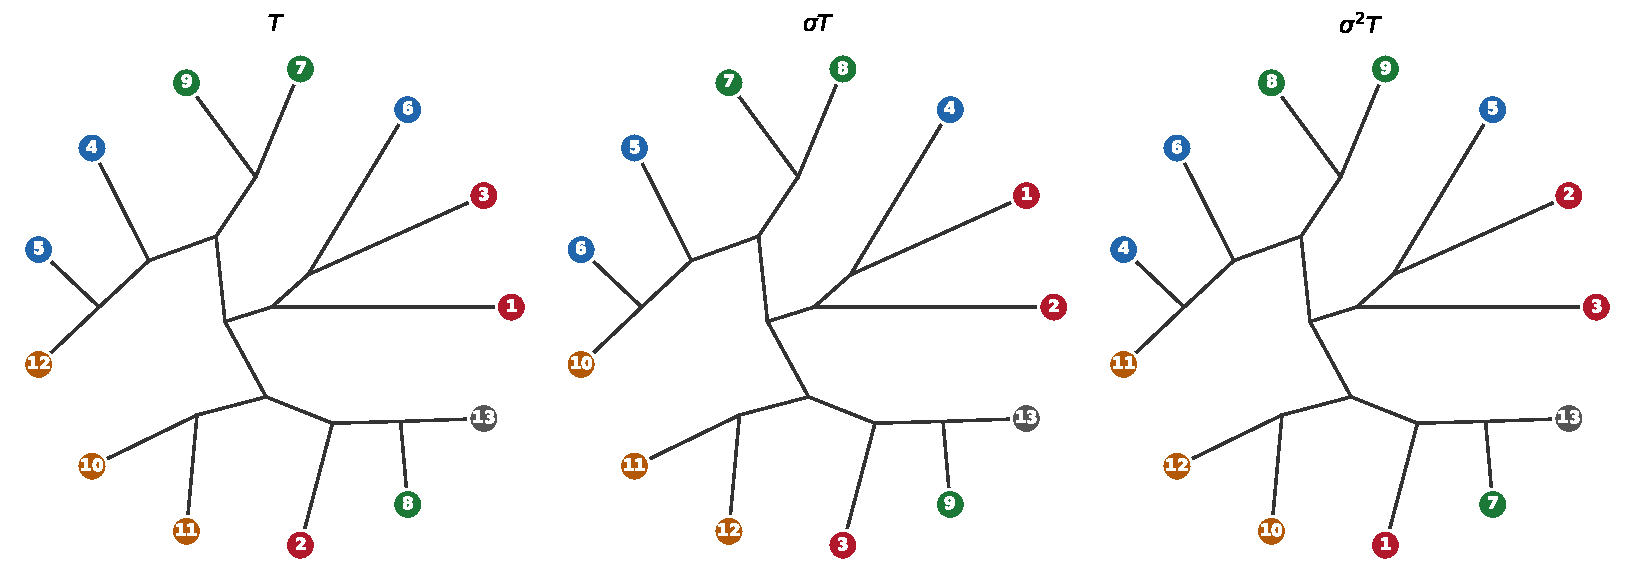
\includegraphics[width=\textwidth]{triple13.pdf}
\caption{The trees $T$, $\sigma T$, $\sigma^2 T$ of Proposition~\ref{prop:lower} in one layout. Colours mark the $\sigma$-orbits $\{1,2,3\}$, $\{4,5,6\}$, $\{7,8,9\}$, $\{10,11,12\}$ and $\{13\}$. No four leaves are split the same way in all three drawings.}
\label{fig:triple}
\end{figure}

The tree was found by a SAT search in which $T$ is the only free tree (Section~\ref{sec:sat}). On thirteen leaves the cycle types $3^41$ and $6^21$ of $\sigma$ admit solutions, while $13$, $12\,1$, $5^23$ and $4^31$ do not. On fourteen leaves the types $3^41^2$, $3^42$, $6^21^2$ and $14$ admit none, in line with Theorem~\ref{thm:h3}.

\subsection*{Fourteen leaves}
The upper bound $h(3)\le14$ is the instance $n=14$ of Snir and Yuster's three-tree separation theorem, whose most technical ingredient is a two-tree lemma with set sizes $4n/27$ and $4n/9$~\cite[Lemma~2.6]{SY2026}, proved with real weights and then stated in an error-free form in their Section~4. At $n=14$ that error-free form asserts exactly Lemma~\ref{lem:two} below. We prove a stronger statement, Lemma~\ref{lem:bip}, by an exhaustive check that takes about a minute, and Lemma~\ref{lem:two} separately by a certified SAT computation, so that $h(3)\le14$ rests on an exact finite argument checked in two independent ways.

\begin{lemma}\label{lem:quartetsep}
Let $X,Y$ be disjoint leaf sets of a tree $T$ with $|X|,|Y|\ge2$. They are separated in $T$ if and only if $T$ resolves $xx'|yy'$ for all distinct $x,x'\in X$ and distinct $y,y'\in Y$.
\end{lemma}

\begin{proof}
One direction was noted above. If $X$ and $Y$ are not separated, the subtrees spanned by $X$ and by $Y$ share a vertex $v$, which is internal. Let $C_1,C_2,C_3$ be the components of $T-v$; each of $X$ and $Y$ meets at least two of them. Take $x\in X\cap C_1$ and $x'\in X\cap C_2$. If $Y$ meets $C_3$, take $y\in Y\cap C_3$ and $y'\in Y\cap(C_1\cup C_2)$; then $y'$ is paired with $x$ or $x'$. Otherwise take $y\in Y\cap C_1$ and $y'\in Y\cap C_2$, giving $xy|x'y'$. Either way $xx'|yy'$ fails.
\end{proof}

\begin{lemma}[computer-assisted, Section~\ref{sec:sat}]\label{lem:two}
Any two phylogenetic trees on $[14]$ have disjoint leaf sets $X,Y$ with $\{|X|,|Y|\}=\{3,4\}$ separated in both.
\end{lemma}

\begin{lemma}[exhaustive check]\label{lem:bip}
Let $[14]=X\cup Y$ with $X\cap Y=\emptyset$ and $|X|,|Y|\ge5$, and let $T$ be a tree on $[14]$. Then some edge of $T$ splits $[14]$ into $Z$ and $W$ such that one of the pairs $(X\cap Z,Y\cap W)$ and $(X\cap W,Y\cap Z)$ consists of a set of at least three and a set of at least four elements. On $13$ leaves the same statement holds when $\{|X|,|Y|\}=\{6,7\}$ and fails when $\{|X|,|Y|\}=\{5,8\}$.
\end{lemma}

\begin{proof}
Relabelling is free, so it suffices to take every unrooted shape on $14$ leaves (there are $135$) and every choice of $5$, $6$ or $7$ of its leaves as $X$, and to inspect all edges: $135\cdot(2002+3003+3432)=1{,}138{,}995$ cases, none without such an edge. On $13$ leaves the $66$ shapes give no failure for $|X|=6$ and $891$ failures for $|X|=5$. The script \texttt{bipartition\_check.py} uses only the standard library.
\end{proof}

\begin{proof}[Proof of Theorem~\ref{thm:h3}]
The lower bound is Proposition~\ref{prop:lower}. Given three trees on $14$ leaves, Lemma~\ref{lem:centroid} gives an edge of $T_1$ splitting $[14]$ into $X,Y$ with $|X|,|Y|\ge5$, and Lemma~\ref{lem:bip} applied to $T_2$ gives sets $X'\subseteq X$ and $Y'\subseteq Y$ separated in $T_1$ and $T_2$ with $\{|X'|,|Y'|\}=\{3,4\}$ after shrinking (Lemma~\ref{lem:two} gives such sets directly). Lemma~\ref{lem:centroid} applied to $T_3|(X'\cup Y')$ gives an edge of $T_3$ splitting these seven leaves into $W,Z$ with $|W|,|Z|\ge3$, and Lemma~\ref{lem:step} with $t=2$ applied to $X',Y'$ gives two sets of at least two leaves separated in all three trees.
\end{proof}

Lemma~\ref{lem:two} is sharp: by Proposition~\ref{prop:lower} and the proof above it fails on thirteen leaves, and a brute-force search confirms that no two of $T,\sigma T,\sigma^2T$ have separated sets of sizes three and four.

\section{\texorpdfstring{Lower bounds for general $k$}{Lower bounds for general k}}\label{sec:lowerbounds}

A linear order of leaves specifies a caterpillar (reversal and swaps within the two end cherries give the same tree), and it splits a $4$-set into the two leaves that come first and the two that come last. Let $L=2^{k-1}$ and $m=2L+1$. For $1\le j\le L$ call $\{j,\,m+1-j\}$ the $j$-th layer, and call $L+1$ the centre. For $t=0,\dots,k-1$ let $C_t$ be the caterpillar whose order has, at position $j$, the element $j$ if $\beta_t(j)=0$ and $m+1-j$ if $\beta_t(j)=1$, the centre at position $L+1$, and the other element of layer $j$ at position $m+1-j$. Here $\beta_0\equiv0$ and $\beta_t(j)$ is binary digit $t-1$ of $j-1$; thus $C_t$ flips the layers $j$ whose digit $t-1$ of $j-1$ is one.

\begin{proposition}\label{prop:cat}
The caterpillars $C_0,\dots,C_{k-1}$ on $2^k+1$ leaves have no common quartet. Hence $h(k)\ge h^*(k)\ge2^k+2$.
\end{proposition}

\begin{proof}
Induction on $k$; for $k=1$ there are three leaves. In every order each layer occupies positions $j$ and $m+1-j$, so the elements of the outer layers $1,\dots,L/2$ always occupy the first and last $L/2$ positions, and the inner layers and the centre always occupy the middle block. In $C_{k-1}$ every inner layer is flipped and no outer layer is, so its order is that of $C_0$ with the middle block reversed. Restricted to the inner layers and the centre, and also restricted to the outer layers and the centre, the orders of $C_0,\dots,C_{k-2}$ form the family for $k-1$ after relabelling, since only digit $k-2$ of $j-1$ distinguishes the two halves. Let $Q$ be a $4$-set.

If $Q$ lies in the inner block, or in the outer layers together with the centre, induction applies. If $Q$ has three outer elements and one inner element $x$, replacing $x$ by the centre changes no split, because both lie in the middle block in every order. If $Q$ has one outer element $o$, then $o$ is first or last in every order and pairs with the inner element nearest to it; this element differs between $C_0$ and $C_{k-1}$, since the middle block is reversed and $Q$ has three inner elements. If $Q$ has two outer elements $o_1,o_2$ and two inner elements, then when $o_1$ and $o_2$ are on opposite sides they pair with different inner elements in $C_0$ and $C_{k-1}$. Otherwise they are on the same side in $C_0$, so they lie in different layers $j_1\ne j_2$ and are both the smaller or both the larger element of their layers; choose a digit in which $j_1-1$ and $j_2-1$ differ, so that exactly one of the two layers is flipped in the corresponding $C_t$. In $C_t$ the elements $o_1,o_2$ are on opposite sides, so $C_t$ splits $Q$ differently from $C_0$. At $k=2$ there is only one outer layer, so this same-side subcase is empty.
\end{proof}

For $k=3$ the orders are $123456789$, $183654729$ and $127654389$; Snir and Yuster~\cite[Sec.~5]{SY2026} list the same three caterpillars. A standard-library script checks Proposition~\ref{prop:cat} directly for $k\le6$. For $k=4$ the bound $18$ is weaker than the $23$ from four trees on $22$ leaves found by a symmetric SAT search (Section~\ref{sec:sat}).



\section{Computations}\label{sec:sat}

\emph{Shapes.} Relabelling leaves preserves both properties studied, so the first tree may be a fixed representative of its unlabelled shape. Deleting a leaf of an unrooted shape and rooting at its former neighbour gives a rooted binary shape on one leaf fewer, so the shapes with $n$ leaves come from the rooted shapes with $n-1$ leaves, deduplicated by a canonical form. The counts $2,2,4,6,11,18,37,66,135$ for $n=6,\dots,14$ agree with OEIS A000672~\cite{OEISA000672}, and an independent enumeration by leaf insertion gives the same counts.

\emph{Free trees.} A free tree is encoded by three variables per $4$-set $\{a<b<c<d\}$, for the splits $ab|cd$, $ac|bd$ and $ad|bc$, with an exactly-one constraint; for every $5$-set the five chosen splits must form the quartet system of one of the $15$ binary trees on those five leaves. Every tree satisfies these constraints, so an unsatisfiable formula excludes all trees. By a theorem of Colonius and Schulze~\cite{CS1981} and Bandelt and Dress~\cite{BD1986} the constraints characterise tree quartet systems, but the arguments never rely on this: every satisfying assignment reported here was rebuilt into a tree by leaf insertion and checked directly.

\emph{Lemma~\ref{lem:two}.} With the first tree $T_1$ fixed, add for every edge split $P|Q$ of $T_1$ and all $X\subseteq P$, $Y\subseteq Q$ (or the reverse) with $\{|X|,|Y|\}=\{3,4\}$ a clause stating that one of the $18$ cross quartets $xx'|yy'$ is not chosen in the free tree $T_2$. By Lemma~\ref{lem:quartetsep} the models are exactly the trees $T_2$ that violate the lemma together with $T_1$. All $135$ formulas, with $33{,}033$ variables and between $160{,}668$ and $163{,}020$ clauses, are unsatisfiable. Each was solved by CaDiCaL~3.0.1~\cite{CaDiCaL2} with a DRAT proof, and every proof was verified by DRAT-trim~\cite{DRATtrim}; the proofs total $3.2$ GB and the solving took $2.7$ hours of wall time on a shared machine. The CNF files are regenerated deterministically and their SHA-256 hashes are recorded. A second implementation sharing no code with the first generates the five-leaf patterns from the $15$ labelled trees, enumerates shapes by leaf insertion, forbids the $228$ non-tree patterns by direct clauses and is solved by Kissat~4.0.4~\cite{Kissat}; it also reports all $135$ formulas unsatisfiable. As a positive control, the same encoding on thirteen leaves with $T_1$ of the shape of $T$ is satisfiable, and the decoded second tree has no separated pair of sizes three and four.

\emph{Theorem~\ref{thm:smallk}.} One program (with numpy) computes, level by level, the least $v$ for which $(u,v)$ is $m$-safe, for $u$ up to a bound, and the resulting bounds on $h(k)$. A second program, written separately with the standard library only, reads the claimed table and re-derives every claim used by the stated bounds with its own implementation of the recursion; it rejects the claims $h(4)\le27$ and $h(3)\le14$ when the claimed tables are lowered by one. The recursion was compared with brute-force enumeration of all labelled trees on up to eight leaves for about $1000$ random sets of bad colour counts, with full agreement, and its level-two values $(5,9)$ and $(6,7)$ agree with the exhaustive check of Lemma~\ref{lem:bip}.

\emph{Searches.} For $k$ trees, fixing $T_1$ and leaving $T_2,\dots,T_k$ free, one clause per $4$-set forbids all free trees from taking the split of $T_1$. In the symmetric variant $T$ is the only free tree, the family is $T,\sigma T,\dots,\sigma^{k-1}T$, and for each $4$-set $Q$ and pairing $s$ a clause forbids $T$ from resolving every $\sigma^{-i}Q$ by $\sigma^{-i}s$. As sanity checks the method reproduces $h(2)=6$ and the caterpillar value $h^*(3)=10$ of~\cite{SY2026}, for which all trees are also forbidden to contain three cherries on six leaves. The construction for $k=4$ in Table~\ref{tab:small} comes from a symmetric search with $\sigma$ of cycle type $4^52$ on $22$ leaves and was verified with the standard-library checker; for $k=5$ the same method reached only $27$ leaves, fewer than the $33$ of Proposition~\ref{prop:cat}. On twelve leaves the three-tree formulas with $T_1$ among the first five shapes, including the caterpillar, are unsatisfiable with checked DRAT proofs; thus three trees on twelve leaves, one a caterpillar, always share a quartet, while such triples exist on eleven leaves.

\section{Questions}

The value of $h(4)$ lies between $23$ and $28$. The certified one-pair strategy of Theorem~\ref{thm:smallk} gives $28$. An exploratory variant starting from three branches at a vertex also gave $28$. The supplied verifier establishes the safe pairs used by our upper bounds; it does not certify global optimality among all one-pair strategies. The exponential growth rate of $h(k)$ lies between $2$ and $\beta$. Since $h(3)=14>h^*(3)$ and $h(4)\ge23>h^*(4)$, general trees do better than caterpillars for small $k$; is $h(k)=O(2^k)$? On the upper side, the numerical value $3/\sqrt2$ of the one-pair game suggests that reaching base $2$ needs an argument that tracks more than one separated pair. It would also be interesting to know whether in every triple on thirteen leaves without a common quartet the three trees have the same shape; on twelve leaves there are triples in which they do not.

\section*{Data and code}
The trees, checkers, CNF generators, solver logs and hashes are in the \texttt{verification} directory next to this paper. The Newick checker, the separation checker, the proof executor, the exhaustive check of Lemma~\ref{lem:bip}, the checker for Theorem~\ref{thm:smallk}, the caterpillar check and both CNF generators for Lemma~\ref{lem:two} use only the Python standard library.

\bibliographystyle{plain}
\bibliography{references}
\end{document}
